
\begin{frame}{目录}
        \begin{center}
            \textcolor{NJU_purple}{\Large 第二部分} \\
            \text{\;} \\
            \textcolor{NJU_purple}{\Huge GRU的原理} 
        \end{center}      
    \end{frame}

\begin{frame}{GRU的核心} 
    \begin{itemize}
        \item GRU(Gated Recurrent Unit)由Cho等人在2014年提出,目标是简化LSTM结构,同时保留其门控机制的优势:
        \begin{itemize}
            \item 合并门控:将LSTM的输入门和遗忘门合并为更新门,减少参数数量。
            \item 统一隐藏状态:取消记忆单元,直接通过隐藏状态传递信息,简化计算流程。
        \end{itemize}
        \item GRU的核心是两个门控机制:更新门(Update Gate)和重置门(Reset Gate),通过动态控制信息流动解决长程依赖问题。
        \begin{figure}
            \centering
            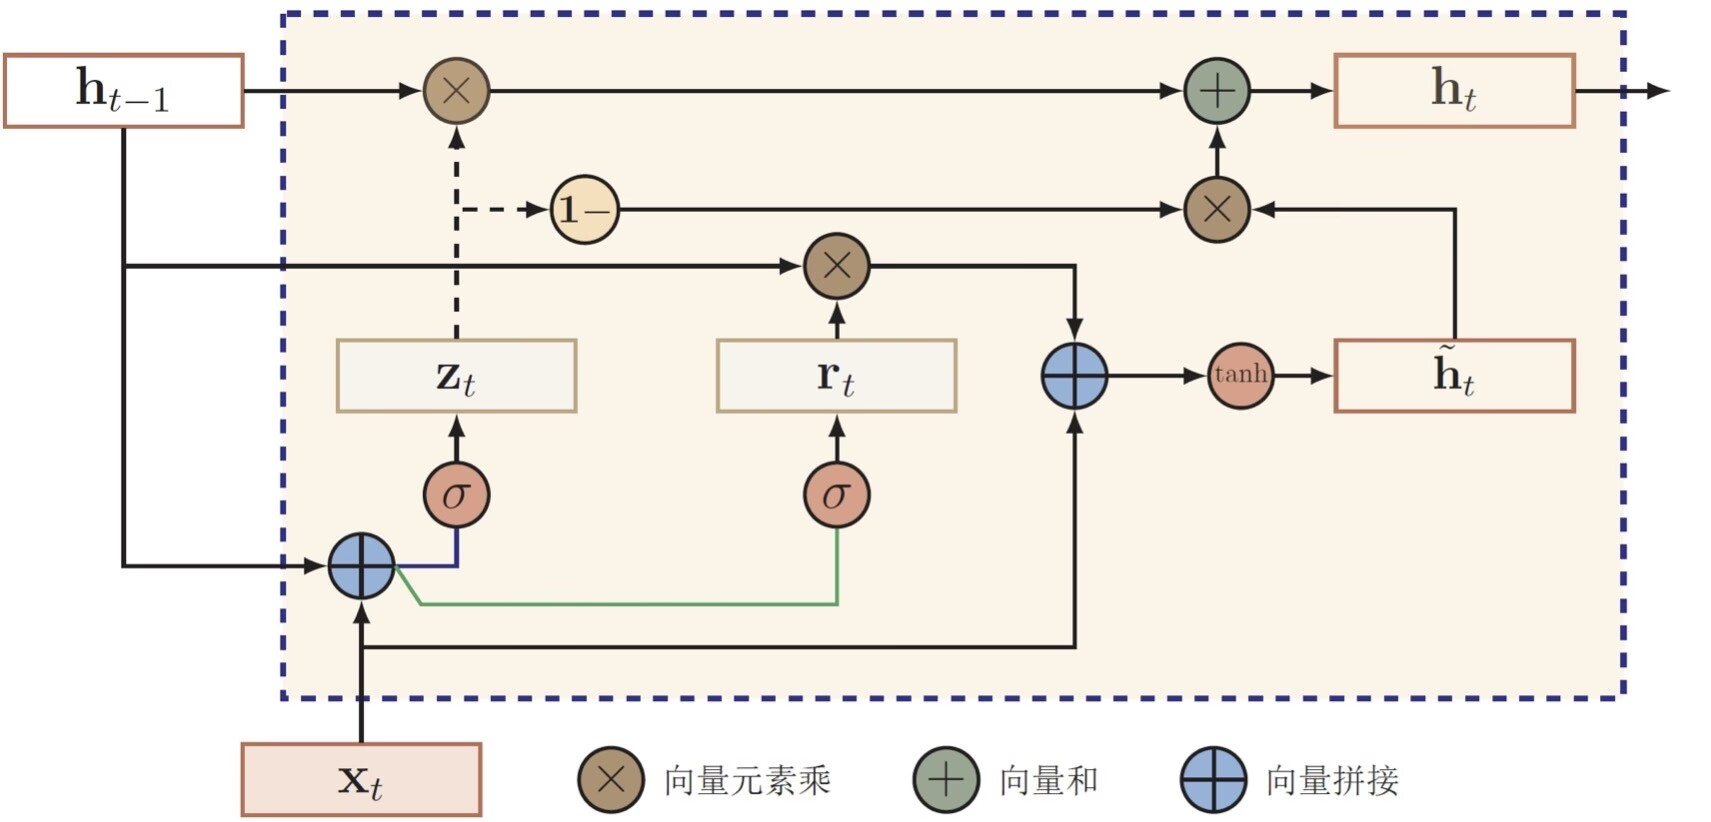
\includegraphics[width=0.55\linewidth]{pic/GRU原理图.png}
            \caption{GRU原理图}
            \label{fig:GRU}
        \end{figure}
    \end{itemize}
\end{frame}

\begin{frame}{GRU的原理:更新门}
    \begin{itemize}
        \item \textbf{更新门}:决定当前时刻隐藏状态应保留多少历史信息,并融合多少新信息。
        \begin{equation*}
            z_t = \sigma(W_z \cdot [h_{t-1},x_t])
        \end{equation*}
        \item 其中,
        \begin{itemize}
            \item \(x_t\)为第\(t\)个时间步的输入向量。
            \item \(W_t\)为权重矩阵。
            \item \(h_{t-1}\)为上一时刻的隐藏状态,即\(t-1\)时间步的信息。
            \item \(\sigma\)为Sigmoid函数,将输出压缩到0 - 1之间。
        \end{itemize}
        \item \(z_t\):更新门的输出(取值0-1),控制历史信息的保留比例。
    \end{itemize}
\end{frame}


\begin{frame}{GRU原理:重置门}
    \begin{itemize}
        \item \textbf{重置门}:决定是否忽略历史信息以生成新的候选状态,即到底遗忘过去的多少信息。
        \begin{equation*}
            r_t = \sigma(W_r \cdot [h_{t-1},x_t])
        \end{equation*}
        \item 其中,
        \begin{itemize}
            \item \(x_t\)为第\(t\)个时间步的输入向量。
            \item \(W_r\)为权重矩阵。
            \item \(h_{t-1}\)为上一时刻的隐藏状态,即\(t-1\)时间步的信息。
            \item \(\sigma\)为Sigmoid函数,将输出压缩到0-1之间。
        \end{itemize}
        \item \(r_t\):重置门的输出(取值0 - 1),接近0时表示忽略历史信息。
    \end{itemize}
\end{frame}


\begin{frame}{GRU原理:候选隐藏状态和隐藏状态更新}
    \begin{itemize}
        \item 候选隐藏状态:结合重置门和历史信息,生成当前时刻的候选状态
        \begin{equation*}
            \tilde{h}_t = tanh(W \cdot [r_t * h_{t-1},x_t])
        \end{equation*}
        \begin{itemize}
            \item \(r_t * h_{t-1}\):重置门控制历史信息的过滤,若\(r_t \approx 0\)则丢弃历史信息,仅依赖当前输入。
        \end{itemize}
        \item 隐藏状态更新:通过更新门融合历史状态和候选状态
        \begin{equation*}
            h_t = (1-z_t) * h_{t-1} + z_t * \tilde{h}_{t-1}
        \end{equation*}
        \begin{itemize}
            \item \(z_t \approx 1\):隐藏状态主要由候选状态更新(关注新信息)。
            \item \(z_t \approx 0\):保留大部分历史信息(忽略当前输入)。
        \end{itemize}
    \end{itemize}
\end{frame}




